\section{加减法数字谜}

\title[第3讲\quad 加减法数字谜]{第3讲\quad 加减法数字谜} 
\author{}
\date{}
\begin{frame}
    \titlepage
\end{frame}

\begin{frame}
    \frametitle{课前测}
    \textit{用0、4、7这三个数字,能组成( )个没有重复数字的三位数.}

    \textit{A.4\\ B.5\\ C.6}
\end{frame}

\begin{frame}
    \frametitle{课前测}
    \textit{用2、4、7、1 组成无重复数字的两位数,可能组成( )个.}

    \textit{A.4\\ B.8\\ C.6}
\end{frame}

\begin{frame}
    \frametitle{课前测}
    \textit{用3、5、0、8 这4张数字卡片摆出的两位数,最小的奇数是多少?}

    \textit{A.30\\ B.33\\ C.35}
\end{frame}



\begin{frame}
    \frametitle{知识梳理}
\end{frame}

\begin{frame}
    \frametitle{MISSION 1}
    \textit{下楼来,金钱卜落;问苍天,人在何方;恨王孙,一直去了;詈冤家,言去不回;悔当初,吾错失口;有上交,无下交;皂白何须问;分开不用刀;从今莫把仇人靠;千种相思撇消!\\
    请问,上面数字谜的谜底是什么?}
\end{frame}

\begin{frame}
    \frametitle{铺垫}
    \textit{相传在很久以前,由于没有很好的防虫措施,书上的算式常常被虫子吃掉一部分,所以人们在看书的时候,就得想办法,根据剩下的算式来判断被吃掉的数是几.后来人们就把这一类问题称为“虫蚀算”。\\
    在空格内填入适当的数字,使加法竖式成立}

    \begin{figure}[H] 
        \centering
        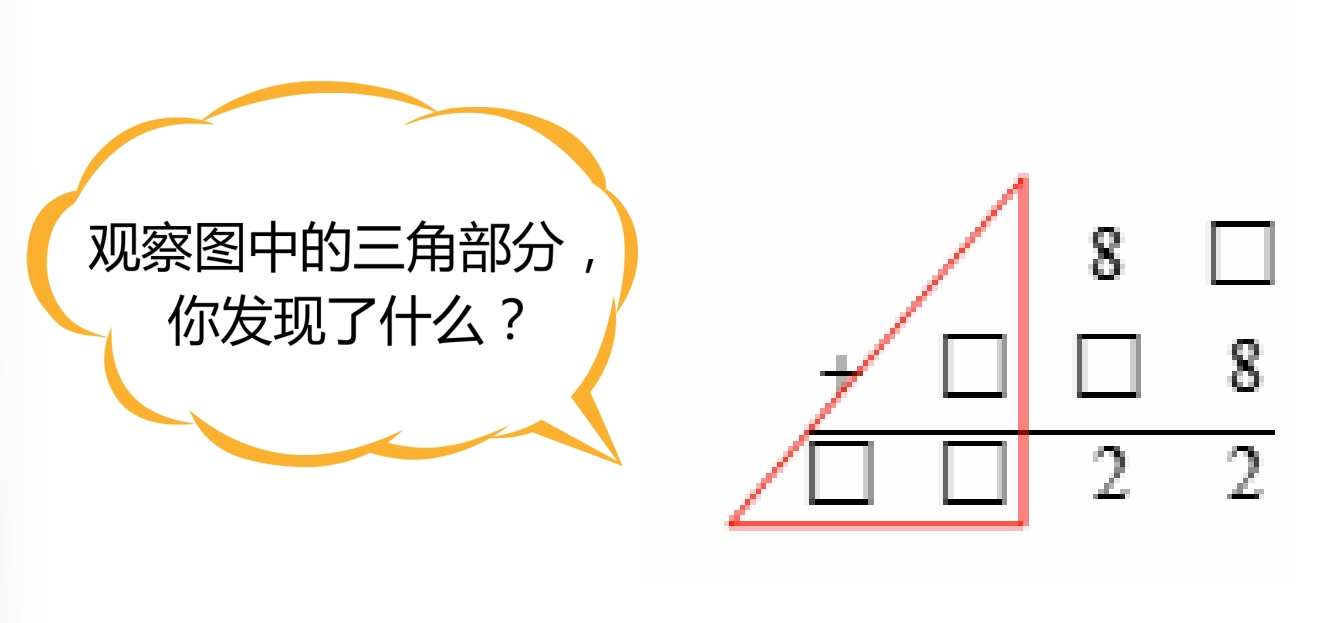
\includegraphics[width=1\textwidth]{./pics/Chapter_3/pudian.png}
    \end{figure}
\end{frame}

\begin{frame}
    \frametitle{探索1}
    \textit{(1)在空格内填入适当的数字,使图中的加法竖式成立.}

    \begin{figure}[H] 
        \centering
        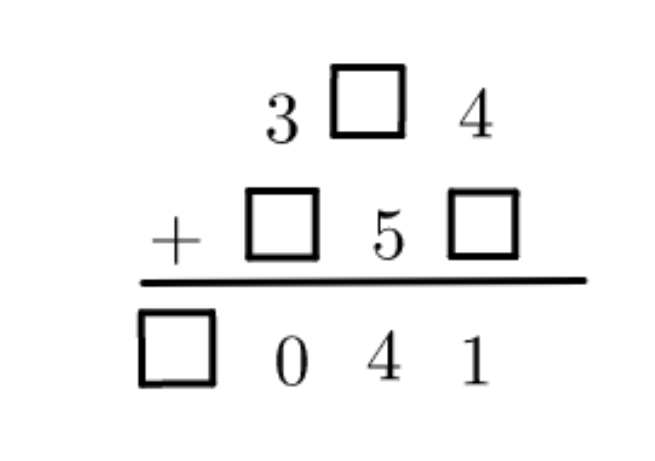
\includegraphics[width=1\textwidth]{./pics/Chapter_3/tansuo1_1.png}
    \end{figure}
\end{frame}

\begin{frame}
    \frametitle{探索1}
    \textit{(2)在空格内填入适当的数字,使图中的减法竖式成立.}

    \begin{figure}[H] 
        \centering
        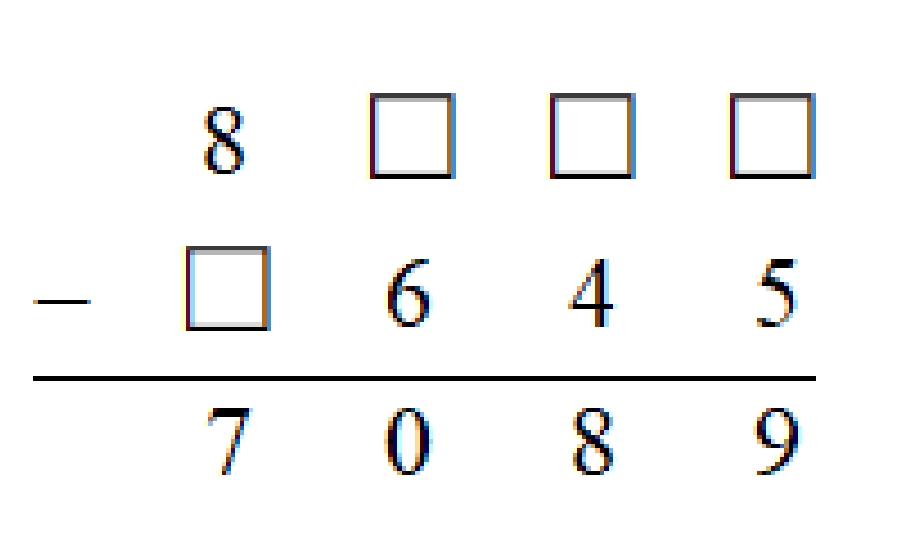
\includegraphics[width=1\textwidth]{./pics/Chapter_3/tansuo1_2.png}
    \end{figure}
\end{frame}

\begin{frame}
    \frametitle{捉虫时刻}
    \textit{请你给企鹅治病,并开出处方。}
    
    \begin{figure}[H] 
        \centering
        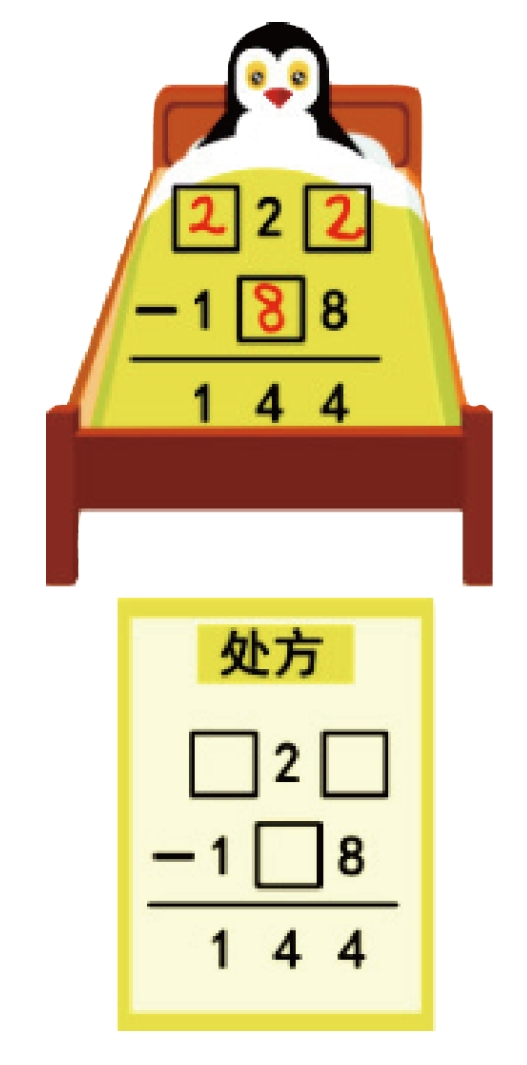
\includegraphics[width=1\textwidth]{./pics/Chapter_3/zhuochong.png}
    \end{figure}
\end{frame}


\begin{frame}
    \frametitle{探索2}
    \textit{(1)在空格内填入适当的数字,使图中的加法竖式成立。}
    
    \begin{figure}[H] 
        \centering
        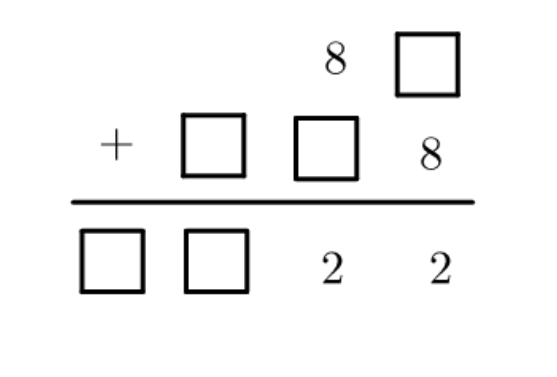
\includegraphics[width=1\textwidth]{./pics/Chapter_3/tansuo2_1.png}
    \end{figure}
\end{frame}

\begin{frame}
    \frametitle{探索2}
    \textit{(2)在空格内填入适当的数字,使图中的加法竖式成立}

    
    \begin{figure}[H] 
        \centering
        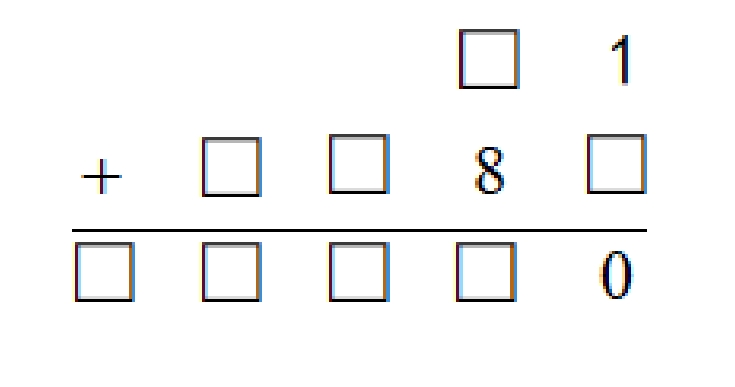
\includegraphics[width=1\textwidth]{./pics/Chapter_3/tansuo2_2.png}
    \end{figure}
\end{frame}

\begin{frame}
    \frametitle{探索3}
    \textit{(1)在空格内填入适当的数字,使图中的减法竖式成立。}
    \begin{figure}[H] 
        \centering
        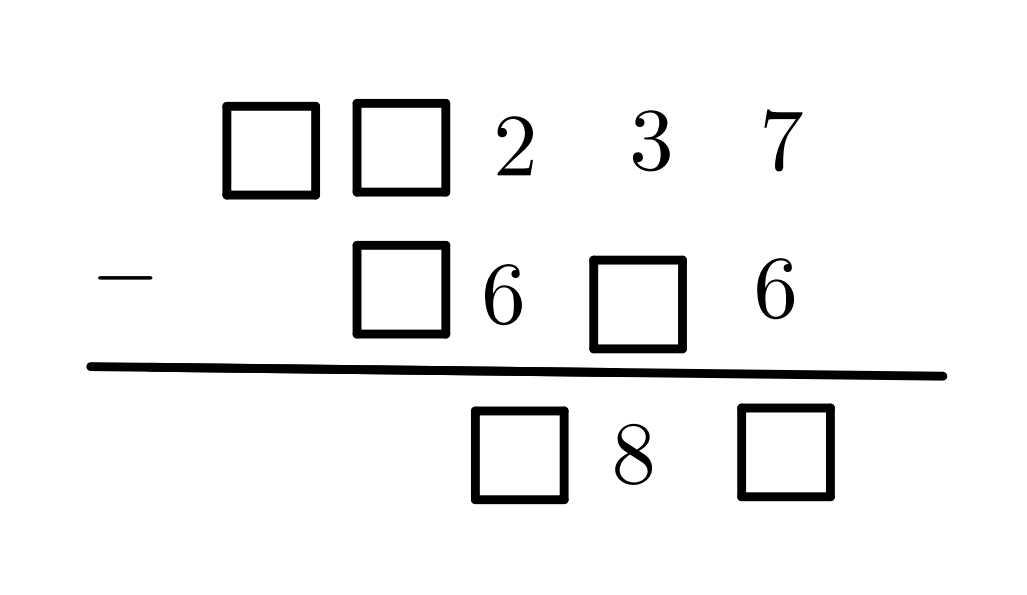
\includegraphics[width=1\textwidth]{./pics/Chapter_3/tansuo3_1.png}
    \end{figure}
\end{frame}

\begin{frame}
    \frametitle{探索3}
    \textit{(2)在空格内填入适当的数字,使图中的减法竖式成立。}
    \begin{figure}[H] 
        \centering
        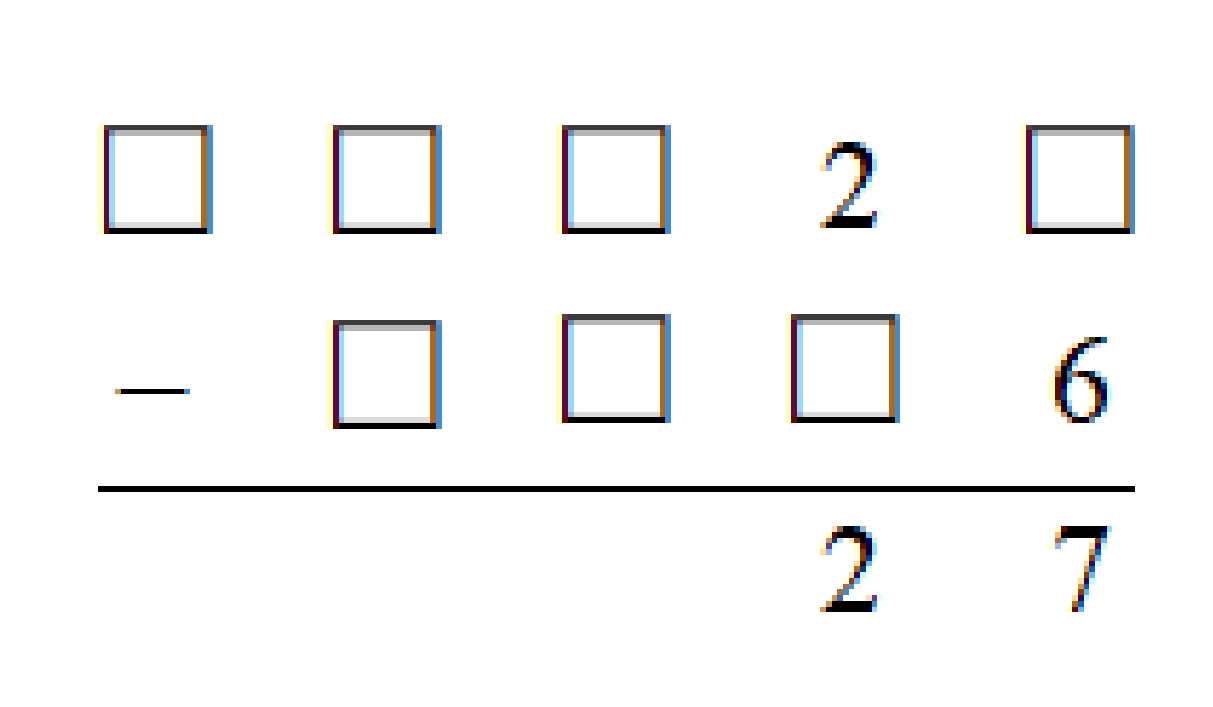
\includegraphics[width=1\textwidth]{./pics/Chapter_3/tansuo3_2.png}
    \end{figure}
\end{frame}


\begin{frame}
    \frametitle{课堂互动1}
    \textit{在下面算式的空格内,各填入一个合适的数字,使算式成立.最后结果是\underline{\hbox to 10mm{}}.}
    \begin{figure}[H] 
        \centering
        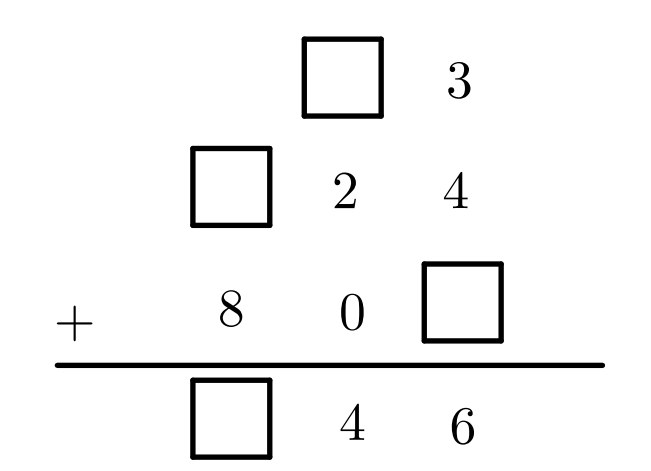
\includegraphics[width=1\textwidth]{./pics/Chapter_3/ketanghudong1.png}
    \end{figure}
\end{frame}

\begin{frame}
    \frametitle{课堂互动2}
    \textit{在下面算式的空格内,填入合适的数字,使算式成立.}
    \begin{figure}[H] 
        \centering
        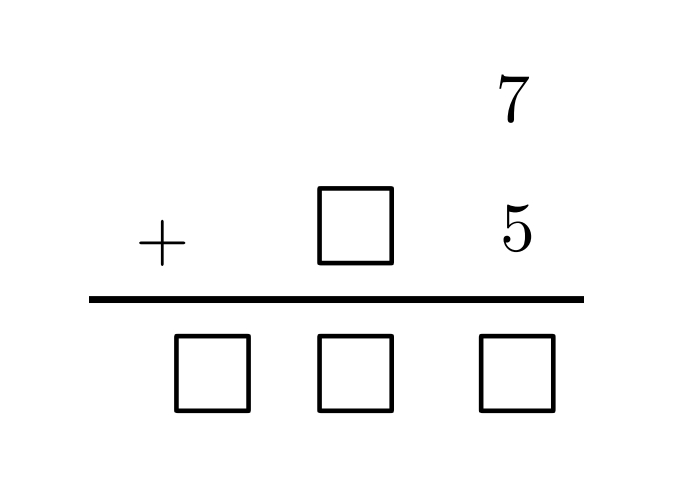
\includegraphics[width=1\textwidth]{./pics/Chapter_3/ketanghudong2.png}
    \end{figure}
\end{frame}

\begin{frame}
    \frametitle{课堂互动3}
    \textit{在下面算式的空格内,填入合适的数字,使算式成立.}
    \begin{figure}[H] 
        \centering
        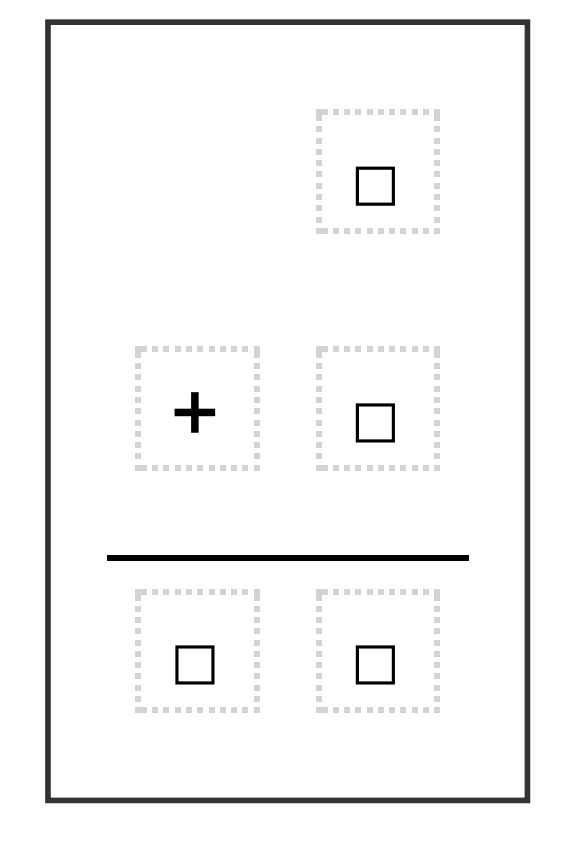
\includegraphics[width=1\textwidth]{./pics/Chapter_3/ketanghudong3.png}
    \end{figure}
\end{frame}


\begin{frame}
    \frametitle{MISSION 2}
    \textit{在数字谜问题中,我们有什么样的分析方法呢?}
\end{frame}


\begin{frame}
    \frametitle{探索4}
    \textit{在下列的算式中,相同的符号代表相同的数字,不同的符号代表不同的数字,根据这个算式,可以推算出: $\square + \bigcirc + \triangle +$ \ding{73} $=$\underline{\hbox to 10mm{}}}
    \begin{figure}[H] 
        \centering
        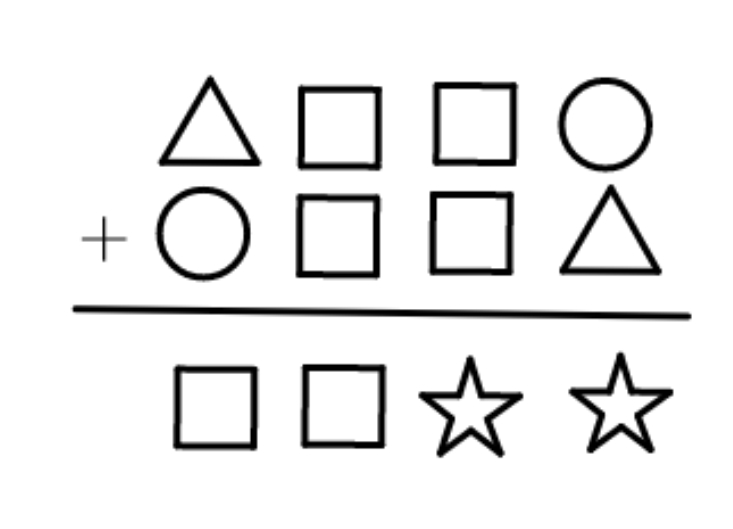
\includegraphics[width=0.5\textwidth]{./pics/Chapter_3/tansuo4.png}
    \end{figure}
\end{frame}

\begin{frame}
    \frametitle{探索5}
    \textit{在下面算式中,相同的字母代表相同的数字,不同的字母代表不同的数字,那么A=\underline{\hbox to 10mm{}}, 
    B=\underline{\hbox to 10mm{}},C=\underline{\hbox to 10mm{}},D=\underline{\hbox to 10mm{}}}
    \begin{figure}[H] 
        \centering
        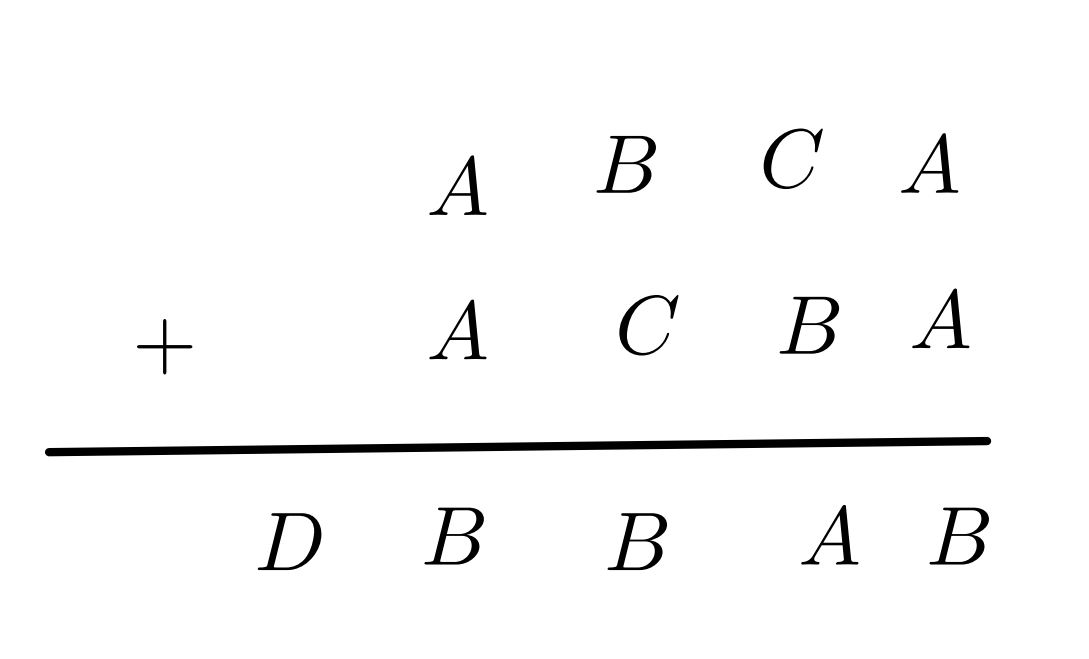
\includegraphics[width=0.5\textwidth]{./pics/Chapter_3/tansuo5.png}
    \end{figure}
\end{frame}




%%%%%%%%%%%%%%%%%%%%%


\begin{frame}
    \frametitle{课堂互动1}
    \begin{figure}[H] 
        \centering
        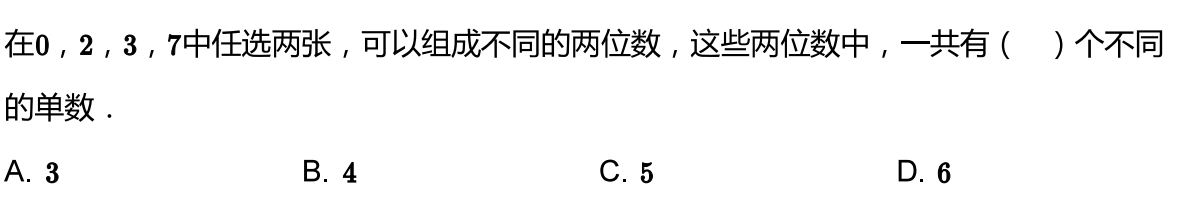
\includegraphics[width=1\textwidth]{./pics/Chapter_2/ketanghudong1.png}
    \end{figure}
\end{frame}

\begin{frame}
    \frametitle{课堂互动2}
    \begin{figure}[H] 
        \centering
        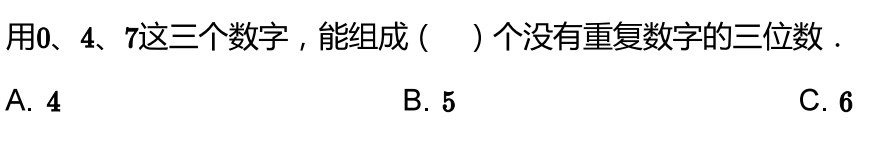
\includegraphics[width=1\textwidth]{./pics/Chapter_2/ketanghudong2.png}
    \end{figure}
\end{frame}

\begin{frame}
    \frametitle{课堂互动3}
    \begin{figure}[H] 
        \centering
        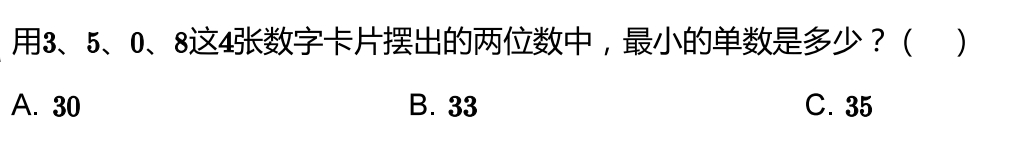
\includegraphics[width=1\textwidth]{./pics/Chapter_2/ketanghudong3.png}
    \end{figure}
\end{frame}





\begin{frame}
    \frametitle{探索5}
    \textit{艾迪去儿童餐厅买15元特惠套餐,他有若干张1元、2元、5元的纸币,但是购买特惠套餐的条件是必须找出一共有多少种不同的付钱方法(要求每种纸币都有),眼看优惠时间就要截止了,同学们你能帮助艾迪顺利买到优惠套餐吗 ?}
\end{frame}

\begin{frame}
    \frametitle{探索6}
    \textit{在某地有四种不同面值的硬币,如图所示,假若你恰有这四种硬币各1枚。问:共能组成多少种不同的钱数?}
    \begin{figure}[H] 
        \centering
        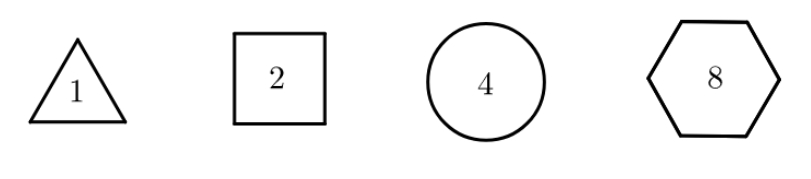
\includegraphics[width=0.5\textwidth]{./pics/Chapter_2/tansuo6.png}
    \end{figure}
\end{frame}

\begin{frame}
    \frametitle{补充1}
    \textit{薇儿收集到四种不同的面值的硬币各1枚,如图所示,一共可以组成多少种不同的钱数?}
    \begin{figure}[H] 
        \centering
        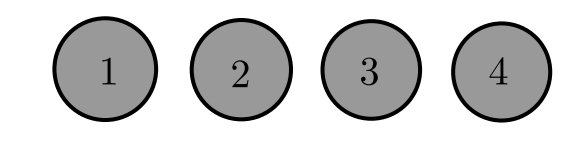
\includegraphics[width=0.3\textwidth]{./pics/Chapter_2/buchong1_1.png}
    \end{figure}
\end{frame}

\begin{frame}
    \frametitle{补充1}
    \textit{艾迪收到三种不同面值的硬币,如图所示,假若你恰好有以下四枚硬币.问共能组成多少种不同的钱数?}
    \begin{figure}[H] 
        \centering
        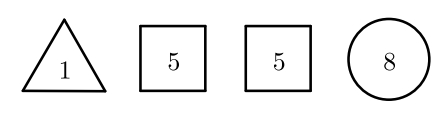
\includegraphics[width=0.3\textwidth]{./pics/Chapter_2/buchong1_2.png}
    \end{figure}
\end{frame}


\begin{frame}
    \frametitle{补充1}
    \textit{用四种不同的硬币各1枚,如图所示,两两一组,一共可以组成多少种不同的钱数?}
    \begin{figure}[H] 
        \centering
        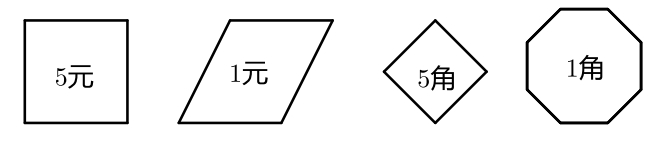
\includegraphics[width=0.3\textwidth]{./pics/Chapter_2/buchong1_3.png}
    \end{figure}
\end{frame}

\begin{frame}
    \frametitle{探索7}
    \textit{博士给艾迪与薇儿上课,课上介绍了``拐弯''的概念.\\
    博士:``对于一行数,如果有三个数abc依次排一起,且a >b,c>b或者a <b,c<b,我们就称它发生了一次拐弯''\\
    艾迪:``我懂了,比如4321没有拐弯,像1243就发生了一次拐弯''\\
    薇儿:``没错,再比如1324就发生了两次拐弯.''\\
    博士:``非常棒!看来你们都掌握得非常扎实了,现在我要考考你们了,如果我们将1,2,3,4排成一行,则能使这行数刚好发生两次拐弯的排列方法共有多少种?''}
\end{frame}

\begin{frame}
    \frametitle{探索8}
    \textit{一次,齐王与田忌赛马,每人各有等级不同的4匹马,这8匹马按照从快到慢的排序分别是齐王的一等马,田忌的一等马,齐王的二等马,田忌的二等马,齐王的三等马,田忌的三等马,齐王的四等马,田忌的四等马.田忌已经提前知道齐王本次赛马的出场顺序是一等、二等、三等、四等,他可以安排种不同的出场顺序,才能保证自己至少战平齐王呢?同学们,你们能帮田忌找出所有可能的决策吗 ?}
\end{frame}

\begin{frame}
    \frametitle{补充2}
    \textit{加加与减减做游戏,两人轮流在一张白纸上写出一个数字,组成一个多位数的前2位,而这个多位数从第三个数字开始,每个数字都恰好是它前面两个数字之和,直至不能再写为止.例如加加减减写了1和4,那么这个多位数就是1459,则这类多位数共有多少个?}
\end{frame}

\begin{frame}
    \frametitle{补充2}
    \textit{如果一个数的各位数字从左到右构成等差数串,我们就称这个数为“跳跃数”,例如:1358642均是“跳跃数”,153就不是“跳跃数”,那么一共有多少个三位“跳跃数”?}
\end{frame}

\begin{frame}
    \frametitle{补充2}
    \begin{figure}[H] 
        \centering
        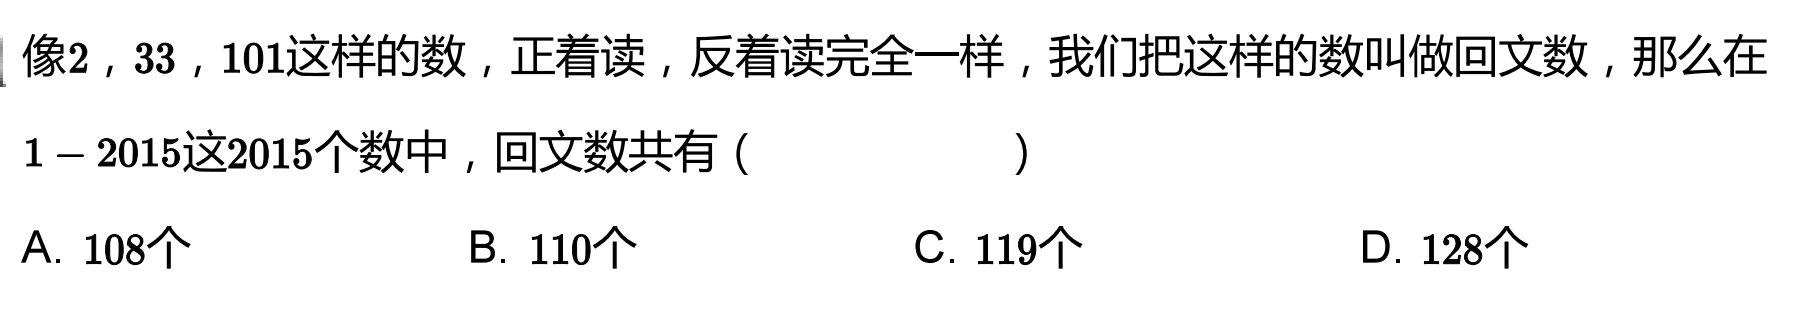
\includegraphics[width=1\textwidth]{./pics/Chapter_2/buchong2_3.png}
    \end{figure}
\end{frame}